\documentclass[12pt]{article}
\usepackage{tikz}
\usetikzlibrary{arrows, shapes, math}
\usepackage{pgfmath}
\usepackage{tkz-euclide}
\usepackage{setspace}
\usepackage{amsmath}
\usepackage{array}
\usepackage{hyperref}
\usepackage{enumerate}
\usepackage{enumitem}
\setlist{noitemsep}
\usepackage{listings}
\usepackage{ragged2e}
\usepackage{tabbing}
\input{arduinoLanguage.tex}
\usepackage{url}


\definecolor{mygreen}{rgb}{0,0.6,0}
\definecolor{mygray}{rgb}{0.5,0.5,0.5}
\definecolor{mymauve}{rgb}{0.58,0,0.82}
\lstset{ %
  backgroundcolor=\color{white},   % choose the background color
%  basicstyle=\footnotesize,        % size of fonts used for the code
  breaklines=true,                 % automatic line breaking only at whitespace
  captionpos=b,                    % sets the caption-position to bottom
  commentstyle=\color{mygreen},    % comment style
  escapeinside={\%*}{*)},          % if you want to add LaTeX within your code
  keywordstyle=\color{blue},       % keyword style
  language=Python,
  stringstyle=\color{mymauve},     % string literal style
}

\usepackage{makeidx}
\usepackage{verbatim}
\usepackage{datetime}
\usepackage[cal=boondoxo]{mathalfa}
\usepackage{longtable}

\setlength{\pdfpageheight}{11in}
\setlength{\textheight}{9in}
\setlength{\voffset}{-1in}
\setlength{\oddsidemargin}{0pt}
\setlength{\marginparsep}{0pt}
\setlength{\marginparwidth}{0pt}
\setlength{\marginparpush}{0pt}
\setlength{\textwidth}{6.5in}

\pagestyle{plain}
\makeindex

\title{Campus Automation Using RFID Technology}
\author{Charles Beam \\ Faculty Mentor: Sanjeetha Peters \\ Subject Area Reader: Randy Key \\ Reader: Dr. Emily Allen}
\newdateformat{vardate}{\THEDAY\ \monthname[\THEMONTH]\ \THEYEAR}
\vardate
\date{\today}

\begin{document}
\setlength{\parindent}{0pt}
\begin{spacing}{1.2}
\setcounter{section}{-1}
\begin{centering}
\huge
\textbf{Campus Automation Using RFID Technology}
\\[0.4in]
\Large
By Charles Beam
\\[0.4in]
\normalsize
Spring 2021
\\[0.8in]
\rule{3in}{0.4pt} \\
Sanjeetha Peters, Senior Lecturer of Mathematics and Computer Science
\\[0.8in]
\rule{3in}{0.4pt} \\
Professor Randy Key, Associate Lecturer of Mathematics
\\[0.8in]
\rule{3in}{0.4pt} \\
Dr. Emily Allen, Associate Lecturer of English
\\[0.8in]
\rule{3in}{0.4pt} \\
Dr. Kristi Key, Director of Academic Services \\
\end{centering}
\newpage
\tableofcontents
\newpage

%%%%%%%%%
\section{General Project Overview}

%%%%%%%%%
\subsection{Purpose}

The purpose of this project is to have students be able to declare their current location. Students do this by having RFID tags that they scan whenever they want to declare their location. Students scan their tags on boxes that are placed around campus where students would need to declare their locations. The RFID box sends these RFID tag scans to a MySQL database for later parsing.

%%%%%%%%%
\subsection{Use Cases}

Some use cases of this project are:
\begin{itemize}
	\item Automating Classroom Attendance
	\item Automating SISO
	\item Automating Speed Bump
	\item Automating Community Meeting Sign In
	\item Automating Activity Attendance (Dance Recitals, Food Servings, Blue and Gold Week Presentations)
\end{itemize}

%%%%%%%%%
\subsection{Importance of Project}

Many required activities at LSMSA are either inefficient or not Covid friendly.
\begin{itemize}
	\item Classroom attendance takes too long. LSMSA, having 262 classes meeting 2.5 times a week for 32 weeks a year means that attendance is taken 20,960 times a year.
	\begin{center} 262 classes * 2.5 meetings/week * 32 weeks = 20,960 attendances taken \end{center}
Assuming that taking attendance takes one minute per class period, teachers spend 350 hours or 14.5 days per school year taking attendance. Attendance on a year-long scale takes far too much time and needs to be automated so teachers can do what they do best, teach.
	\begin{center} 20,960 attendances/year * 1 minute = 20,960 minutes / 349.33 hours / 14.56 days \end{center}
	\item The current solution for student locations (SISO using Reach) is a clunky, expensive mess. Students rarely update it with their actual locations, there is no method to ensure students are being honest, and Reach does not consistently work among many other issues.
	\item Currently, speed bumping students requires the students to stand at the front desks of the dorms and make sure that the front desk worker sees them. If the front desk worker misses them, the student has to go down at 7 pm to speed bump again. This means multiple students are all walking to the desk at the same time, which is not good for social distancing.
	\item For community meetings, students wait outside the doors and slowly walk in getting their IDs scanned. This is not a good system since it is not only slow, but makes students group together allowing for Covid to travel between them.
	\item For food events or events happening in the Recital Hall, students have to sign a sheet of paper stating that they are there. To do this, students all use the same pen and paper, which is not good for preventing germs from spreading.
\end{itemize}

%%%%%%%%%
\section{Hardware Overview}

This project has three main pieces of hardware, all communicating with each other to successfully scan student's RFID IDs.

%%%%%%%%%
\subsection{RFID Box}

RFID Boxes are physically placed at locations where students need to declare their locations. Inside the boxes are two boards communicating with each other: the NodeMCU ESP-12E and the RC522.

%%%%%%%%%
\subsubsection{NodeMCU ESP-12E}
\begin{center}
\includegraphics[height=5cm]{esp-12e.jpg}
\end{center}
The NodeMCU ESP-12E is the brain of the RFID box. Essentially, a NodeMCU ESP-12E is an Arduino with a WiFi chip built-in. This allows it to run Arduino code to interact with the RC522 but also be able to communicate with the MySQL database through the school's WiFi.
\newline\newline
The NodeMCU ESP-12E also has a blue LED (like a small light bulb) built-in. This LED provides the user with confirmation whenever they scan their RFID ID.
%%%%%%%%%
\subsubsection{RFID Reader RC522}
\begin{center}
\includegraphics[height=5cm]{RC522.jpg}
\end{center}
The RC522 is the board that reads the RFID tags. Whenever a RFID tag is scanned, the contents of the tag are sent to the NodeMCU ESP-12E.

%%%%%%%%%
\subsection{RFID Tag}
\begin{center}
\includegraphics[height=5cm]{RFID Tag.png}
\end{center}
A RFID tag contains an ID that is transmitted to the RC522 when in close proximity. Each student is issued one RFID tag.

%%%%%%%%%
\section{Software Overview}

This project has two main pieces of software: The program on the NodeMCU ESP-12E and the MySQL Database. These two pieces of software communicate with each other over the school's WiFi.

%%%%%%%%%
\subsection{NodeMCU ESP-12E Program Overview}

%%%%%%%%%
\subsubsection{Program Flowchart}
	\Large
	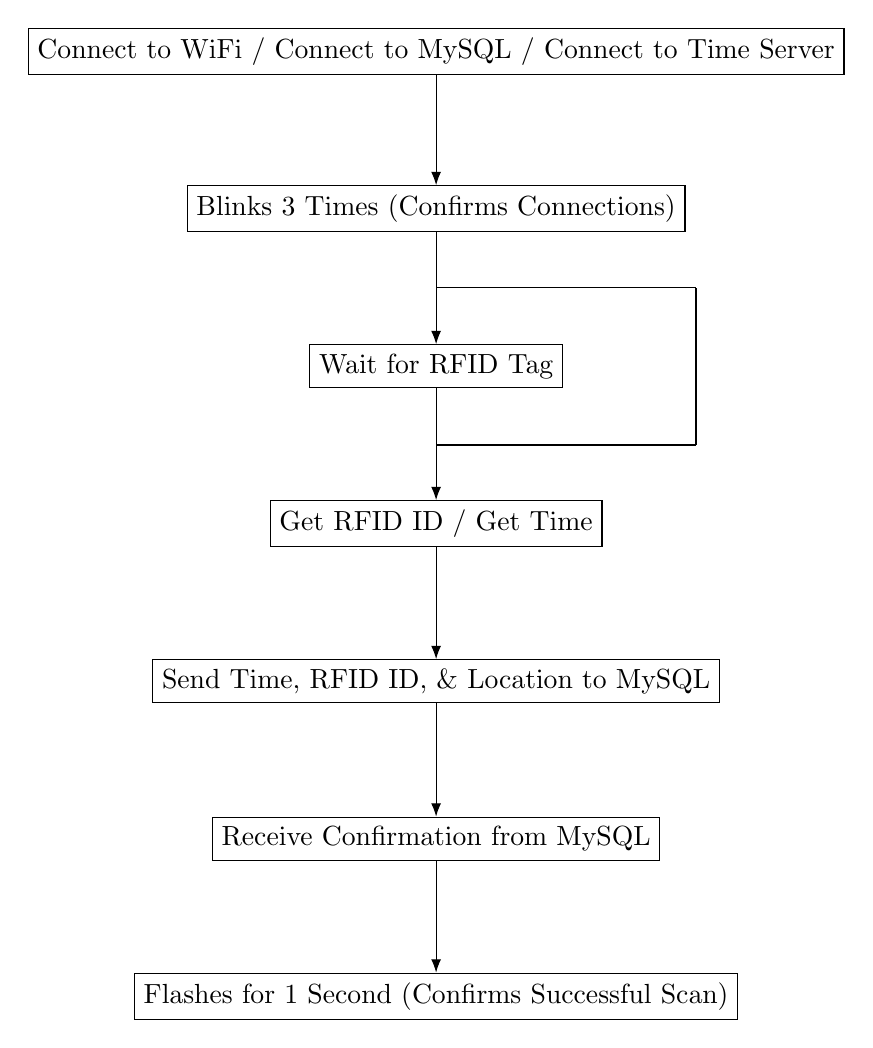
\begin{tikzpicture}[x=11mm, y=20mm,yscale=1]
		\node (a) at (0,0)[draw, rectangle, align=center]{Connect to WiFi / Connect to MySQL / Connect to Time Server};
		\node (b) at (0,-1)[draw, rectangle, align=center]{Blinks 3 Times (Confirms Connections)};
		\node (c) at (0,-2)[draw, rectangle, align=center]{Wait for RFID Tag};
		\node (d) at (0,-3)[draw, rectangle, align=center]{Get RFID ID / Get Time};
		\node (e) at (0,-4)[draw, rectangle, align=center]{Send Time, RFID ID, \& Location to MySQL};
		\node (f) at (0,-5)[draw, rectangle, align=center]{Receive Confirmation from MySQL};
		\node (g) at (0,-6)[draw, rectangle, align=center]{Flashes for 1 Second (Confirms Successful Scan)};
		\foreach \i/\j in {a/b, b/c, c/d, d/e, e/f, f/g}
			\draw [-Latex] (\i) -- (\j);
		\draw (c) -- (0,-2.5);
		\draw (0,-2.5) -- (3,-2.5);
		\draw (3,-2.5) -- (3,-1.5);
		\draw (3,-1.5) -- (0,-1.5);
		
	\end{tikzpicture}
\normalsize
%%%%%%%%%
\subsubsection{Entire Program}
Descriptions of each part of this program is found in the next section.
\begin{lstlisting}[language=Arduino]  
#include <SPI.h>
#include <MFRC522.h>
#include <ESP8266WiFi.h>
#include <MySQL_Connection.h>
#include <MySQL_Cursor.h>
#include <NTPClient.h>
#include <WiFiUdp.h>

#define RST_PIN         D3 
#define SS_PIN          D8
IPAddress server_addr(MySQL IP Address (Replace periods with commas));  // IP of the MySQL database
char user[] = "MySQL Username";             // MySQL Username
char password[] = "MySQL Password";       // MySQL Password
char ssid[] = "WiFi Username";        		// WiFi Username
char pass[] = "WiFi Password";    	      // WiFi Password
WiFiClient client;
MySQL_Connection conn(&client);
MySQL_Cursor* cursor;

const long utcOffsetInSeconds = -18000;

WiFiUDP ntpUDP;
NTPClient timeClient(ntpUDP, utcOffsetInSeconds);
String timer;
char timerarray[9];
char location[] = "ClassT231";
MFRC522 mfrc522(SS_PIN, RST_PIN);
String uidstring;
char uid[12];
void setup() {

  Serial.begin(115200);
  SPI.begin(); 
  pinMode(LED_BUILTIN, OUTPUT);
  Serial.printf("\nConnecting to %s", ssid);
  WiFi.begin(ssid, pass);
  while (WiFi.status() != WL_CONNECTED) {
    delay(500);
    Serial.print(".");
  }
  Serial.println("\nConnected to network");
  Serial.print("My IP address is: ");
  Serial.println(WiFi.localIP());
  Serial.print("Connecting to SQL...  ");
  if (conn.connect(server_addr, 3306, user, password/*, default_db*/))
    Serial.println("MySQL Connected");
  else
    Serial.println("MySQL Failed");
  

  cursor = new MySQL_Cursor(&conn);
  mfrc522.PCD_Init(); 
  timeClient.begin();
  Serial.println(F("Read personal data on a MIFARE PICC:"));
  if(WL_CONNECTED && conn.connected())
        digitalWrite(LED_BUILTIN, HIGH);
        delay(100);                       
        digitalWrite(LED_BUILTIN, LOW);   
        delay(100);                      
        digitalWrite(LED_BUILTIN, HIGH);  
        delay(100); 
        digitalWrite(LED_BUILTIN, LOW);   
        delay(100);                      
        digitalWrite(LED_BUILTIN, HIGH);  
        delay(100); 
        digitalWrite(LED_BUILTIN, LOW);   
        delay(100);                      
        digitalWrite(LED_BUILTIN, HIGH);  
}

void loop() {

  if ( ! mfrc522.PICC_IsNewCardPresent()) {
    return;
  }

  if ( ! mfrc522.PICC_ReadCardSerial()) {
    return;
  }
  timeClient.update();
  uidstring = String(mfrc522.uid.uidByte[0], HEX) + " " + String(mfrc522.uid.uidByte[1], HEX) + " " + String(mfrc522.uid.uidByte[2], HEX) + " " + String(mfrc522.uid.uidByte[3], HEX);
  uidstring.toUpperCase();
  uidstring.toCharArray(uid, 12);
  timer = (timeClient.getFormattedTime());
  timer.toCharArray(timerarray, 9);
  char INSERT_SQL[50];
  sprintf(INSERT_SQL, "INSERT INTO Classrooms_Prod.%s (timedate, rfid_id, location) VALUES ('%s', '%s', '%s')", location, timerarray, uid, location);
  Serial.println(INSERT_SQL);
  if (conn.connected())
    cursor->execute(INSERT_SQL);
  digitalWrite(LED_BUILTIN, LOW);
  delay(1000);                
  digitalWrite(LED_BUILTIN, HIGH); 
} 
\end{lstlisting}

%%%%%%%%%
\subsubsection{Libraries Used}
\begin{lstlisting}[language=Arduino]  
#include <SPI.h>
#include <MFRC522.h>
#include <ESP8266WiFi.h>           
#include <MySQL_Connection.h>
#include <MySQL_Cursor.h>
#include <NTPClient.h>
#include <WiFiUdp.h>  
\end{lstlisting}
The purpose of importing these libraries is to access functions needed for the RFID boxes to work.
\newline\newline
Line descriptions (purpose of each library):
\begin{enumerate}
	\item Used as interface method for RC522.
	\item Used to access methods needed to interface with RC522.
	\item Used to interface with ESP-12E and access the internet.
	\item Used to connect to MySQL database.
	\item Used to interface with MySQL database.
	\item Used to interface with NTP (time server).
	\item Used to connect with NTP (time server).
\end{enumerate}

%%%%%%%%%
\subsubsection{RFID Reader RC522 Setup}

\begin{lstlisting}[language=Arduino]  
#define RST_PIN         D3          
#define SS_PIN          D8          
MFRC522 mfrc522(SS_PIN, RST_PIN);  
String uidstring;
char uid[12];
\end{lstlisting}

Line descriptions:
\begin{enumerate}
	\item Sets the RST pin used to interface with the RC522. This can be changed if using a board other than NodeMCU ESP-12E.
	\item Sets the SS pin used to interface with the RC522. This can be changed if using a board other than NodeMCU ESP-12E.
	\item Gets the RST and SS pin numbers and creates a RC522 instance.
	\item Creates the unformatted string that the RFID ID is stored on.
	\item Creates the formatted RFID ID char array.
\end{enumerate}

%%%%%%%%%
\subsubsection{WiFi Setup}

\begin{lstlisting}[language=Arduino]  
char ssid[] = "WiFi Username";       	  // WiFi Username
char pass[] = "WiFi Password";    	  // WiFi Password
WiFiClient client;                
\end{lstlisting}

Line descriptions:
\begin{enumerate}
	\item This is the location of the WiFi username. It can be changed to whatever the network's name is. Note: keep the username in the quotation marks. Ex: ``username''.
	\item This is the location of the WiFi password. It can be changed to whatever the network's password is. Note: keep the password in the quotation marks. Ex: ``password''.
	\item Initializes the WiFiClient class.
\end{enumerate}

%%%%%%%%%
\subsubsection{Time Server Setup}

\begin{lstlisting}[language=Arduino]  
WiFiUDP ntpUDP;
const long utcOffsetInSeconds = -18000;
NTPClient timeClient(ntpUDP, utcOffsetInSeconds);
String timer;
char timerarray[9];
\end{lstlisting}

Line descriptions:
\begin{enumerate}
	\item Initializes the WiFiUDP class and declares a ntpUDP object.
	\item Sets the time offset from UTC time. In CST this is -18000 seconds. This can be changed for different time-zones.
	\item Initializes the NTPClient class giving it the ntpUDP object from line 1 and the time offset from line 2.
	\item Creates unformatted string that the time is stored on.
	\item Creates the formatted time char array.
\end{enumerate}

%%%%%%%%%
\subsubsection{Connecting to WiFi}

\begin{lstlisting}[language=Arduino]  
Serial.printf("\nConnecting to %s", ssid);
WiFi.begin(ssid, pass);
 while (WiFi.status() != WL_CONNECTED) {
   delay(500);
   Serial.print(".");
 }
Serial.println("\nConnected to network");
Serial.print("My IP address is: ");
Serial.println(WiFi.localIP());
\end{lstlisting}

Line descriptions:
\begin{enumerate}
	\item Prints to the serial console that it is connecting to WiFi and includes the WiFi username. Nothing is printed whenever the RFID boxes are not connected to a computer.
	\item Connects to WiFi
	\item Starts a loop that stops whenever connected to the WiFi.
	\item Waits 0.5 seconds before moving to the next line. If there is no delay, then ``.....'' would spam the console and make it hard to understand. 
	\item Prints a ``.'' to the serial console for testing.
	\item Ends the loop started in line 3. The only way to get past this line in the program is to have a successful WiFi connection.
	\item Prints to the serial console that the WiFi connection was successful.
	\item Prints to the serial console ``My IP address is: ``.
	\item Prints to the serial console the IP address of the RFID box.
\end{enumerate}

%%%%%%%%%
\subsubsection{Connecting to MySQL Database}

\begin{lstlisting}[language=Arduino]  
IPAddress server_addr(MySQL IP address);
char user[] = "MySQL Username";              // MySQL Username
char password[] = "MySQL Password";        // MySQL Password
char location[] = "ClassT231";
MySQL_Connection conn(&client);
MySQL_Cursor* cursor;
\end{lstlisting}

Line descriptions:
\begin{enumerate}
	\item Declares the IP address of the MySQL database.
	\item This is the location of the MySQL database username. It can be changed to whatever the MySQL
username is. Note: keep the username in the quotation marks. Ex: “admin”.
	\item This is the location of the MySQL database password. It can be changed to whatever the MySQL
password is. Note: keep the password in the quotation marks. Ex: “password”.
	\item This is the location of the RFID box location.
	\item Connects to the MySQL database using the username and password declared in lines 2 and 3.
	\item Sets the location to interface with the MySQL database.
\end{enumerate}

%%%%%%%%%
\subsubsection{Connecting to Time Server}

\begin{lstlisting}[language=Arduino]  
timeClient.begin();
\end{lstlisting}

Line descriptions:
\begin{enumerate}
	\item Connects to the time server.
\end{enumerate}

%%%%%%%%%
\subsubsection{Checking Connection / Startup and Connecting Successful LED Blink}

\begin{lstlisting}[language=Arduino]  
if(WL_CONNECTED && conn.connected()){
      digitalWrite(LED_BUILTIN, HIGH);  
      delay(100);                       
      digitalWrite(LED_BUILTIN, LOW);    
      delay(100);                      
      digitalWrite(LED_BUILTIN, HIGH);  
      delay(100); 
      digitalWrite(LED_BUILTIN, LOW);   
      delay(100);                      
      digitalWrite(LED_BUILTIN, HIGH);  
      delay(100); 
      digitalWrite(LED_BUILTIN, LOW);   
      delay(100);                      
      digitalWrite(LED_BUILTIN, HIGH);  
}
\end{lstlisting}

Line descriptions:
\begin{enumerate}
	\item Checks if the RFID box is successfully connected to the WiFi and MySQL database. The lines after this only run if these connections are successful.
	\item Turns off the LED on the NodeMCU ESP-12E.
	\item Waits 0.1 seconds.
	\item Turns on the LED on the NodeMCU ESP-12E.
	\item Waits 0.1 seconds.
	\item Turns off the LED on the NodeMCU ESP-12E.
	\item Waits 0.1 seconds.
	\item Turns on the LED on the NodeMCU ESP-12E.
	\item Waits 0.1 seconds.
	\item Turns off the LED on the NodeMCU ESP-12E.
	\item Waits 0.1 seconds.
	\item Turns on the LED on the NodeMCU ESP-12E.
	\item Waits 0.1 seconds.
	\item Turns off the LED on the NodeMCU ESP-12E.
	\item Ends the conditional in item 1. Lines after this will run whether the connection was successful or not, as checked in line 1.
\end{enumerate}

%%%%%%%%%
\subsubsection{Waiting for RFID Tag}

\begin{lstlisting}[language=Arduino]  
Serial.println(F("Read personal data on a MIFARE PICC:")); 
void loop() {
  if ( ! mfrc522.PICC_IsNewCardPresent()) {
    return;
  }

  if ( ! mfrc522.PICC_ReadCardSerial()) {
    return;
  }
\end{lstlisting}

Line descriptions:
\begin{enumerate}
	\item Prints to the console that the RFID box is ready to read RFID tags.
	\item Begins the main loop of the program. Everything within this loop runs repeatedly after the setup.
	\item Checks if a new RFID tag is present. Line 4 only runs if this is not true and there is no RFID tag present.
	\item Since there is no RFID tag present, the loop is restarted and the program goes back to line 2.
	\item Ends the if statement from line 3. Everything after this runs only if a new card is present, since if a new card is not present, the loops keeps restarting before getting to this point.
	\item
	\item Checks if the RFID tag is readable. Line 8 only runs if this is not true and the RFID tag is not readable.
	\item Since the RFID tag is not readable, the loop is restated and the program goes back to line 2.
	\item Ends the if statement from line 7. Everything after this runs only the scanned RFID tag is readable. 
\end{enumerate}

%%%%%%%%%
\subsubsection{Retrieve RFID ID and Time}

\begin{lstlisting}[language=Arduino]  
uidstring = String(mfrc522.uid.uidByte[0], HEX)
+ " " + String(mfrc522.uid.uidByte[1], HEX)
+ " " + String(mfrc522.uid.uidByte[2], HEX)
+ " " + String(mfrc522.uid.uidByte[3], HEX);
uidstring.toUpperCase();
uidstring.toCharArray(uid, 12);
timer = (timeClient.getFormattedTime());
timer.toCharArray(timerarray, 9);
\end{lstlisting}

Line descriptions:
\begin{enumerate}
	\item Sets the unformatted RFID ID string to include the first byte (two hexadecimal digits) of data. Note: in the actual program, lines 1-4 are all on the same line. The only reason they are separated in this example for formatting.
	\item Adds a space and the second byte of data to the RFID ID string.
	\item Adds a space and the third byte of data to the RFID ID string.
	\item Adds a space and the fourth byte of data to the RFID ID string.
	\item Sets all the characters in the unformatted RFID ID string to be capital for formatting reasons.
	\item Changes the unformatted RFID ID string to a char array for compatibility with the MySQL library and stores this formatted string in the uid char array.
	\item Retrieves the time from the time server and stores it in the unformatted time string.
	\item Changed the unformatted time string to a char array for compatibility with the MySQL library and stores this formatted string in the timearray char array.
\end{enumerate}

%%%%%%%%%
\subsubsection{Send Time, RFID ID, and Location to MySQL Database}

\begin{lstlisting}[language=Arduino]
char INSERT_SQL[50];
sprintf(INSERT_SQL, "INSERT INTO Classrooms_Prod.%s 
(timedate, rfid_id, location) VALUES ('%s', '%s', '%s')", 
location, timerarray, uid, location);
Serial.println(INSERT_SQL);
if (conn.connected())
  cursor->execute(INSERT_SQL);
\end{lstlisting}

Line descriptions:
\begin{enumerate}
	\item Creates a char array to store the command that will be sent to the MySQL database.
	\item sprintf() allows for the program to insert char arrays into other char arrays. Starts the char array.
	\item Continues the char array.
	\item Gives the method the char arrays for location, time, and RFID ID.
	\item Prints the finished MySQL command to the serial console.
	\item Checks if the MySQL connection is successful. Line 7 only runs if this is true and the connection is successful.
	\item Sends the MySQL command to the database.
\end{enumerate}

%%%%%%%%%
\subsubsection{Confirm Successful Scan with 1 Second Flash}

\begin{lstlisting}[language=Arduino]  
digitalWrite(LED_BUILTIN, LOW);   
delay(1000);              
digitalWrite(LED_BUILTIN, HIGH);  
\end{lstlisting}
The purpose of this section of code is to confirm to the user that their RFID tag has been successfully scanned.
\newline\newline
Line descriptions:
\begin{enumerate}
	\item Turns the LED on.
	\item Waits 1 second.
	\item Turns the LED off.
\end{enumerate}

%%%%%%%%%
\subsection{MySQL Database}

A good way to think of the MySQL database is like an Excel spreadsheet. Here is a picture of the current iteration of the MySQL table:
\begin{center}
\includegraphics[height=7cm]{MySQL Table.png}
\end{center}
The columns in this table represent a type of data, whereas every row represents a different log.

The timedate is the time of the scan, rfid\_id is the RFID ID of the scan, and the location is the location of the scan. The timedate data is in military time to avoid needing am/pm.

%%%%%%%%%
\subsection{Data Connections}

	\LARGE
	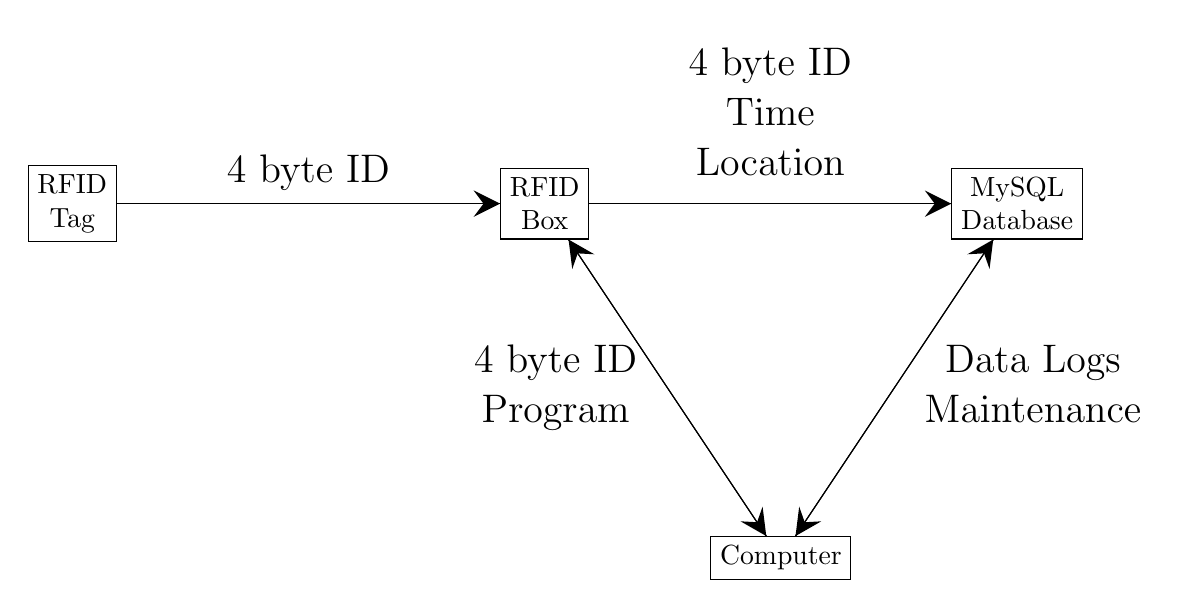
\begin{tikzpicture}[x=20mm, y=30mm, scale = 3]
		\node (t) at (0,0)[draw, rectangle, align=center]{RFID \\ Tag};
		\node (b) at (1,0)[draw, rectangle, align=center]{RFID \\ Box};
		\node (d) at (2,0)[draw, rectangle, align=center]{MySQL \\ Database};
		\node (c) at (1.5,-.5)[draw, rectangle, align=center]{Computer};
		\Large
		\foreach \i/\j/\t/\y/\g in {b/c, d/c}
			\draw [decoration={markings,mark=at position 1 with {\arrow[scale=3,>=stealth]{>}}},postaction={decorate}] (\i) -- (\j);
		\draw [decoration={markings,mark=at position 1 with {\arrow[scale=3,>=stealth]{>}}},postaction={decorate}] (t) -- (b) node [midway, above, xshift=0] {4 byte ID};
		\draw [decoration={markings,mark=at position 1 with {\arrow[scale=3,>=stealth]{>}}},postaction={decorate}] (b) -- (d) node [midway, above, xshift=0] {\begin{tabular}{c} 4 byte ID \\ Time \\ Location \end{tabular}};
		\draw [decoration={markings,mark=at position 1 with {\arrow[scale=3,>=stealth]{>}}},postaction={decorate}] (c) -- (b) node [midway, left, xshift=0] {\begin{tabular}{c} 4 byte ID \\ Program \end{tabular}};
		\draw [decoration={markings,mark=at position 1 with {\arrow[scale=3,>=stealth]{>}}},postaction={decorate}] (c) -- (d) node [midway, right, xshift=0] {\begin{tabular}{c} Data Logs \\ Maintenance \end{tabular}};
	\end{tikzpicture}
	\normalsize
	
	This shows the data that is transferred from and to all the components of this system.

%%%%%%%%%
\section{Buying Parts}

The parts mentioned in the following breakdown were bought on Amazon. Now that the economic effects of the pandemic seem to be over, these parts can be ordered online though a site like Alibaba for much cheaper since the parts would be bought in bulk and straight from a factory.f.

%%%%%%%%%
\subsection{Cost Breakdown}
For an entire project cost breakdown, refer to section \ref{conclusion}.

%%%%%%%%%
\subsubsection{RFID Box}

Single Box Cost:
\begin{center}
\begin{tabular}{ |c c c c|}

\hline
Name & Price & Quantity & Cost\\
\hline \hline
NodeMCU ESP-12E & \$4.67 & 1 & \$4.67 \\
\hline
RC522 & \$2.56 & 1 & \$2.56 \\
\hline
Micro-B Cable & \$1.00 & 1 & \$0.06 \\ 
\hline
M3 12mm Screws & \$0.06 & 4 & \$0.24 \\ 
\hline
M3 Locknuts & \$0.05 & 4 & \$0.20 \\ 
\hline
Box Material & \$0.89 & 1 & \$0.89 \\
\hline
&&&\$8.62 \\
\hline
\end{tabular}
\end{center}

Total cost per RFID box: \$8.62
\newline
If the school wants to use 50 boxes, then the cost would be \$431.

%%%%%%%%%
\subsubsection{RFID Tag}

\label{RFIDTagsCost}
\begin{center}
\begin{tabular}{ |c | c | c | c| }

\hline
Name & Price & Quantity & Cost\\
\hline \hline
13.56MHz  RFID Key Fob Write Only (Black) & \$0.18 & 360 & \$64.80 \\
\hline
\end{tabular}
\end{center}

Total cost per RFID tag: \$0.18
\newline
Assuming the school has 360 , then the cost for all RFID tags would be \$64.80.

%%%%%%%%%
\subsubsection{MySQL Database}
\begin{center}
\begin{tabular}{ |c c c c| }

\hline
Name & Price & Quantity & Cost\\
\hline \hline
db.t2.micro & \$0.0116/hr & 12 Months/12hrs a day & \$50.81 \\
\hline
\end{tabular}
\end{center}

Total Cost of Database: \$50.81 per year

%%%%%%%%%
\subsection{Where to Buy Parts}

%%%%%%%%%
\subsubsection{NodeMCU ESP-12E}

\url{https://www.amazon.com/HiLetgo-Internet-Development-Wireless-Micropython/dp/B081CSJV2V/ref=sr_1_3?dchild=1&keywords=nodemcu+esp12e&qid=1614801567&sr=8-3}

%%%%%%%%%
\subsubsection{RFID Reader RC522}

\url{https://www.amazon.com/Qunqi-Sensor-Module-Arduino-Raspberry/dp/B07QBPGYBF/ref=sr_1_4?dchild=1&keywords=rc522&qid=1614801411&sr=8-4}

%%%%%%%%%
\subsubsection{Micro-B Cable}

\url{https://www.dollartree.com/e-circuit-micro-usb-cables-39-in/259578}

%%%%%%%%%
\subsubsection{M3 12mm Screws}

\url{https://www.amazon.com/Uxcell-a15070200ux0058-Stainless-Phillips-Screws/dp/B012TE1TBS/ref=sr_1_5?dchild=1&keywords=m3+x+12+screw&qid=1619772138&sr=8-5}

%%%%%%%%%
\subsubsection{M3 Locknuts}

\url{https://www.amazon.com/100Pcs-Stainless-Self-Lock-Inserted-Clinching/dp/B075ZZW7VL/ref=sr_1_3?dchild=1&keywords=m3+locknut&qid=1619772083&sr=8-3}

%%%%%%%%%
\subsubsection{3D Printing Filament for RFID Box Case}

\url{https://www.microcenter.com/product/485634/inland-175mm-black-pla-3d-printer-filament-1kg-spool-(22-lbs)}

%%%%%%%%%
\subsubsection{RFID Tag}

\url{https://www.amazon.com/gp/product/B0897KHNHV/ref=ppx_yo_dt_b_asin_title_o07_s00?ie=UTF8&psc=1}

%%%%%%%%%
\subsubsection{MySQL Database}

\url{https://aws.amazon.com/rds/mysql/}

%%%%%%%%%
\section{RFID Box Setup}

%%%%%%%%%
\subsection{Printing RFID Box Case}

Print the RFID box case with support turned on. The other settings do not matter.

%%%%%%%%%
\subsection{Soldering RC522}

An eight pin long straight row pin is soldered on so that it is easy to connect the RC522 to NodeMCU ESP-12E
\begin{center}
\includegraphics[height=5cm, angle=90]{Soldering Pins Bottom.jpg} \\
Bottom of RC522 to show soldering. \\
The pins are soldered on the bottom. \\
\includegraphics[height=5cm, angle = -90]{Soldering Pins Top.jpg} \\
Top of RC522 to show where the long side of pins should be. \\
The long end of the pins come out of the top. \\
\end{center}

%%%%%%%%%
\subsection{Wiring RC522 with NodeMCU ESP-12E}

Using jumper wires or 22 AWG wires. The exact method does not matter as long as these pins are connected:

\begin{center}
\begin{tabular}{ |c c c| }
\hline
RC522 & $\longrightarrow$ & Node ESP-12E \\
\hline \hline
3.3V & $\longrightarrow$ & 3.3V \\
\hline
RST & $\longrightarrow$ & D3 \\
\hline
GND & $\longrightarrow$ & GND \\
\hline
IRQ & $\longrightarrow$ & Not Connected \\
\hline
MISO & $\longrightarrow$ & D6 \\
\hline
MOSI & $\longrightarrow$ & D7 \\ 
\hline
SCK & $\longrightarrow$ & D5 \\
\hline
SS & $\longrightarrow$ & D8 \\
\hline
\end{tabular}
\end{center}

Pictures of Wiring:
\begin{center}
\includegraphics[height=5cm]{RC522 Pinout.jpg}\\
RC522 pinout \\
\includegraphics[height=5cm]{NodeMCU Pinout.jpg} \\
NodeMCU ESP-12E pinout \\
\end{center}

%%%%%%%%%
\subsection{Setting Up Arduino Software}\label{programming box}

Open up the Nodemcu\_Program.ino file.

The screen should look like this:

\begin{center}
\includegraphics[height=10cm]{Arduino Program.PNG}
\end{center}

Make sure that the board selected is NodeMCU 1.0 (ESP-12E Module).

\begin{center}
\includegraphics[height=10cm]{Arduino Program 2.PNG}
\end{center}

Make sure that the correct port is selected. This may take a couple tries to get the correct port.

\begin{center}
\includegraphics[height=10cm]{Arduino Program 3.PNG}
\end{center}

Next, click the upload button in the top left corner. Before uploading the program, make sure that the WiFi, location, and MySQL are all set up.

\begin{center}
\includegraphics[height=10cm]{Arduino Program 4.PNG}
\end{center}

If everything went successfully, the console should print ``Wrote 287584 bytes (209254 compressed) at 0x00000000 in 18.7 seconds (effective 123.2 kbit/s)... \\
Hash of data verified.'' and look like:

\begin{center}
\includegraphics[height=10cm]{Arduino Program 5.PNG}
\end{center}

%%%%%%%%%
\subsubsection{Configuring WiFi}

Insert the WiFi username and password into the two fields below:

Keep the quotation marks around the username and password.
\begin{lstlisting}[language=Arduino]
char ssid[] = "WiFi Username";
char pass[] = "WiFi Password";
\end{lstlisting}


%%%%%%%%%
\subsubsection{Configuring Location}

Insert the RFID box's location into the field below:

Keep the quotation marks around the location.

\begin{lstlisting}[language=Arduino]
char location[] = "location"; 
\end{lstlisting}

%%%%%%%%%
\subsubsection{Configuring MySQL Database Connection}

Insert the MySQL IP Address, username, and password into the three fields below:

Keep the quotation marks around the username and password.
In the MySQL IP address exchange the periods for commas. Ex: 192,54,563,654 when the IP is 192.54.563.654.
\begin{lstlisting}[language=Arduino]
IPAddress server_addr(IP Address); 
char user[] = "MySQL Username";    
char password[] = "MySQL Password'';   
\end{lstlisting}

%%%%%%%%%
\subsection{Testing Box}

Once the program is uploaded, open the serial monitor. The following should appear:

\begin{center}
\includegraphics[height=10cm]{Serial.PNG}
\end{center}

If there is an error, repeat the process and ensure the WiFi, location, and MySQL are all correctly configured.

%%%%%%%%%
\section{RFID Tag Setup}

Open the rfid\_read\_personal\_data.ino example file for the MRFC522 library. Load the program onto a box and scan a RFID tag. 

\begin{center}
\includegraphics[height=10cm]{Serial 2.PNG}
\end{center}

The data after ``Card UID: `` is the RFID tag ID. In this example the ID is ``FA 69 AE B2''.

%%%%%%%%%
\section{MySQL Database Setup}

In MySQL Workbench run these commands:
\begin{itemize}
	\item CREATE DATABASE Classrooms\_Prod;
	\item USE Classrooms\_Prod;
\end{itemize}
This creates a database on the MySQL server and selects it for further commands.

%%%%%%%%%
\section{Adding a Location}

Run these commands:
\begin{itemize}
	\item USE Classrooms\_Prod;
	\item CREATE TABLE ``location name'' (
	\item timedate VARCHAR(20) PRIMARY KEY,
	\item rfid\_id TEXT NOT NULL,
	\item location TEXT NOT NULL
	\item )
\end{itemize}

Change ``location name'' with the name of the location. Do not include the ``''. This should be the same location name that is in the Arduino program.


%%%%%%%%%
\section{Remove a Location}

Run these commands:
\begin{itemize}
	\item DROP TABLE ``location''
\end{itemize}

Change ``location name'' with the name of the location. Do not include the ``''. This should be the same location name that is in the Arduino program.

%%%%%%%%%
\section{Future of Project}

This project is far from being finished. The items in this section would make the project more complete and a better system. In the future, the items in this section would be added to the system.

%%%%%%%%%
\subsection{Redundancy}

Having redundancy in a system like this is paramount. In a normal attendance system, the redundancy is to write student names down on a piece of paper. While this can be a final layer of redundancy for this system as well, it would be better to have a faster solution. Also, considering that this system has many pieces, there needs to be redundancy for each piece.
\newline\newline
We need redundancy for these scenarios:
\begin{enumerate}
	\item A student loses their RFID tag
	\item A RFID box breaks
	\item The MySQL database doesn't respond
	\item Attendance gets entered incorrectly
\end{enumerate}

%%%%%%%%%
\subsubsection{RFID Tag Backup}

Students can easily lose their RFID tag if it falls off their lanyard or breaks. Students should have a person they can go to who can assign them a new RFID tag and update their tag ID in the system. The good news is that this is not a long or complicated process, just not implemented yet.

%%%%%%%%%
\subsubsection{RFID Box Backup}

\Large
	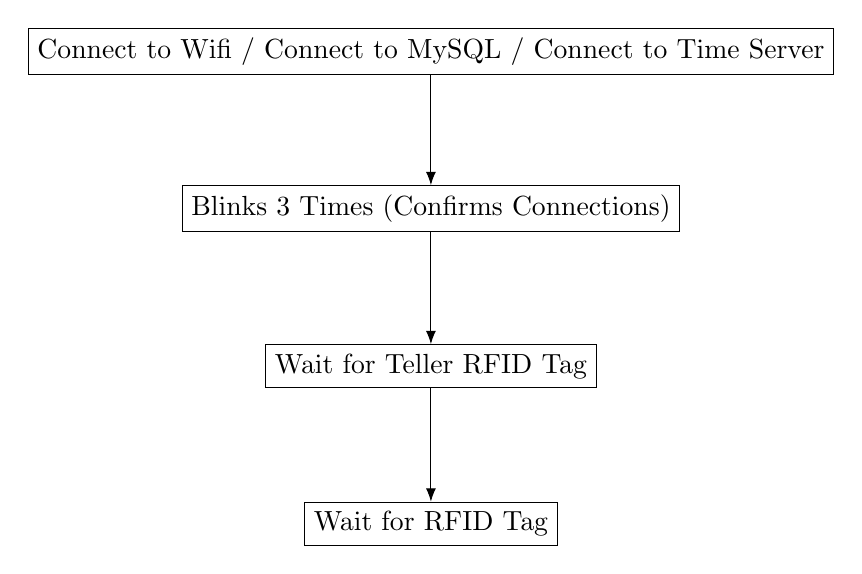
\begin{tikzpicture}[x=11mm, y=20mm,yscale=1]
		\node (a) at (0,0)[draw, rectangle, align=center]{Connect to Wifi / Connect to MySQL / Connect to Time Server};
		\node (b) at (0,-1)[draw, rectangle, align=center]{Blinks 3 Times (Confirms Connections)};
		\node (b2) at (0,-2)[draw, rectangle, align=center]{Wait for Teller RFID Tag};
		\node (c) at (0,-3)[draw, rectangle, align=center]{Wait for RFID Tag};
		\foreach \i/\j in {a/b, b/b2, b2/c}
			\draw [-Latex] (\i) -- (\j);
		
	\end{tikzpicture}
\normalsize

The addition to the project here is that during the setup phase (before the RFID box waits for a RFID Tag) the RFID box waits for a teller tag. This teller tag will have a location ID on it. The RFID box uses this location ID to set its current location. These backup RFID boxes would be in common areas near classrooms for easy access. The RFID teller tags would be left on a desk or on a wall hook in each location. Having backup RFID boxes ensures that if a box is to break, then there is a quick and easy backup minimizing downtime for the system.

%%%%%%%%%
\subsubsection{MySQL Database Backup}

\Large
	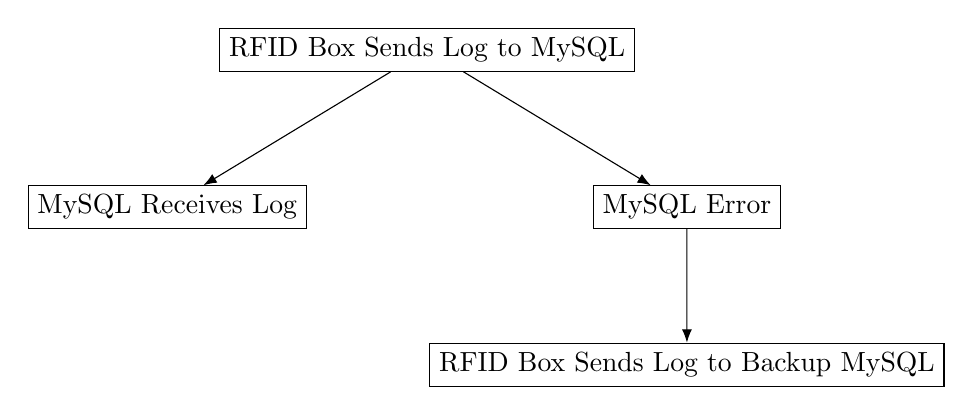
\begin{tikzpicture}[x=11mm, y=20mm, xscale = 3]
		\node (a) at (0,0)[draw, rectangle, align=center]{RFID Box Sends Log to MySQL};
		\node (b) at (-1,-1)[draw, rectangle, align=center]{MySQL Receives Log};
		\node (c) at (1,-1)[draw, rectangle, align=center]{MySQL Error};
		\node (d) at (1,-2)[draw, rectangle, align=center]{RFID Box Sends Log to Backup MySQL};
		\foreach \i/\j in {a/b, a/c, c/d}
			\draw [-Latex] (\i) -- (\j);
	\end{tikzpicture}
\normalsize

The addition to the project here is that there is two possibilities after the RFID box tries to send a location log to the MySQL database. In the current iteration of this project, if a log fails to send, nothing happens. In this new iteration, if this happens, then the RFID box would send the log to a different MySQL database. Having this ability allows for the box to have a much lower chance of failing to send a location log.

%%%%%%%%%
\subsubsection{Attendance Correction}

\Large	
	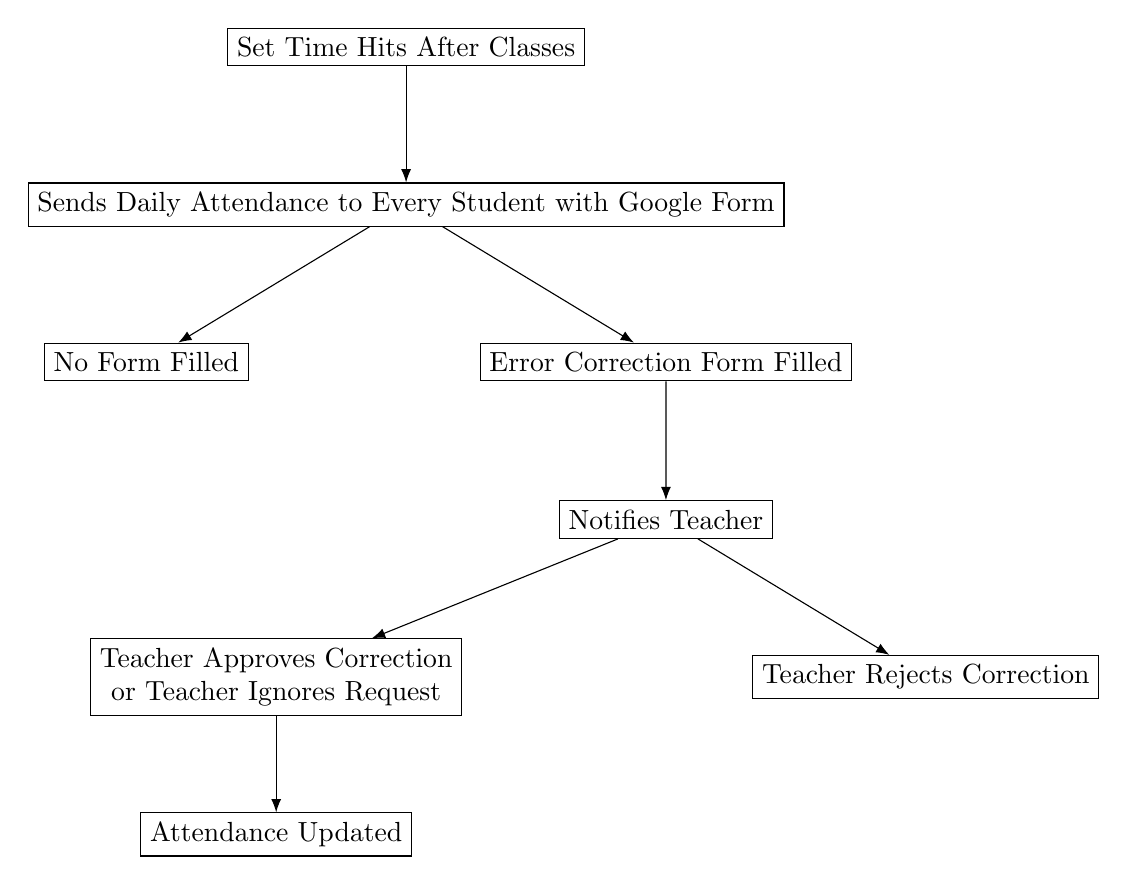
\begin{tikzpicture}[x=11mm, y=20mm,yscale=1, xscale = 3]
		\node (a) at (0,0)[draw, rectangle, align=center]{Set Time Hits After Classes};
		\node (b) at (0,-1)[draw, rectangle, align=center]{Sends Daily Attendance to Every Student with Google Form};
		\node (c) at (-1,-2)[draw, rectangle, align=center]{No Form Filled};
		\node (d) at (1,-2)[draw, rectangle, align=center]{Error Correction Form Filled};
		\node (e) at (1,-3)[draw, rectangle, align=center]{Notifies Teacher};
		\node (f) at (-0.5,-4)[draw, rectangle, align=center]{Teacher Approves Correction \\ or Teacher Ignores Request};
		\node (g) at (-0.5,-5)[draw, rectangle, align=center]{Attendance Updated};
		\node (h) at (2,-4)[draw, rectangle, align=center]{Teacher Rejects Correction};
		
		\foreach \i/\j in {a/b, b/c, b/d, d/e, e/f, f/g, e/h}
			\draw [-Latex] (\i) -- (\j);
	\end{tikzpicture}
\normalsize

The addition to the project here is that students have the ability to correct a wrong attendance log. For example, if two RFID boxes get mixed up somehow or a student's RFID tag fails to read, then the attendance will still be correct. If a student's attendance is wrong, they can fill out a google form. This form's data is parsed through and another email is sent to teachers asking them if the attendance correction is correct. There are two possibilities at this point. If the teacher approves the correction or ignores the email, then the attendance correction is assumed to be correct and the attendance logs are updated. On the other hand, if the teacher rejects the correction, then the attendance correction is assumed to be incorrect, and the attendance logs are not updated.

%%%%%%%%%
\subsection{RFID Box Wall Holder}

One problem with the current implementation of this project is that students might have troubles getting their RFID tags close enough to the RFID boxes to get a read. A solution to this problem would be having a wall holder for each RFID box.
\newline\newline
There are two possible implementations of this solution:
\newline\newline
Implementation 1 would be to have a command strip hook that would be stuck to the wall. The RFID boxes would have a hole in the back of them to hang on the command hooks. This is a good option for temporary setup since the command hooks can be taken down easily.
\newline\newline
Implementation 2 would be to have a sleeve that is screwed into the wall. The RFID box would be inserted into this sleeve. This is the better option for long term implementation. One of the downsides of this is that since the RFID sleeves are screwed into the wall, it is hard to change the position of them.
\newline\newline
The best solution would likely be a mix of both implementations with implementation two being used more for classrooms and building entrances where the positions are constant and implementation one being used for events where the locations are not always the same. 

%%%%%%%%%
\subsection{Injection Molded Case}

Although having a 3D printed case is good for rapid prototyping, having the case be injection molded would have many benefits.
\begin{itemize}
	\item Cheaper (in bulk)
	\item Faster to produce
	\item Less work needed (current box needs to have 3D printing support removed)
	\item Stronger
	\item Does not wear down as fast
	\item Stays clean longer (space between 3D printing lines can collect dust)
\end{itemize}

%%%%%%%%%
\subsection{BlackBaud Integration}

BlackBaud is the backend for many school systems. This project could interface with BlackBaud using BlackBaud's API. The location logs could be downloaded and parsed by python, which would send the data to BlackBaud.

%%%%%%%%%
\subsection{Downloading Data at Night}

At night, all of the data from the MySQL database could be downloaded. This will allow for there to be a backup of the data and allow for the data to be parsed. 

%%%%%%%%%
\subsection{Clips Inside for RFID Reader RC522}

Currently, the RC522 board is aligned using pins in the model. However, it would be much nicer and last longer if clips were added to the model to secure the board down.

%%%%%%%%%
\subsection{Automating Textbook Check-Out}

If textbooks were each given a RFID sticker, students could quickly grab textbooks, scan them, then scan their ID and the system could automatically check out the textbook to the student. This would allow for the textbook checkout and return process to go much faster.

%%%%%%%%%
\section{Conclusion} \label{conclusion}
To conclude, this project has massive potential for speeding up everyday school processes and ensuring that students do not crowd together or share common items. \\ I personally feel that if this gets implemented at a school, the following effects could be achieved:
\begin{itemize}
	\item Teachers would have more time to teach since they no longer need to take attendance.
	\item Student would get sick less due to not being as crowded and sharing less items.
	\item Processes like speed bumping and signing into events would go faster/smoother. 
\end{itemize}
For the low cost of \$546.61 the first year and \$50.81 each subsequent year, implementing this system is very cost effective considering teachers spend 350 hours a year on attendance alone and many hours speed bumping and other processes where students declare their location. \\

Assuming this system is used for attendance since the time taken is easy to calculate the cost would be: \\
\begin{itemize}
	\item First Year: \$1.56 per hour saved
	\item Subsequent Years: \$0.145 per hour saved
\end{itemize}
%%%%%%%%%%%%%%%%
\end{spacing}
\end{document}